\documentclass[9.5pt]{article}
\renewcommand{\baselinestretch}{1.3} 
\renewcommand{\thefootnote}{\alph{footnote}}
\setlength{\parskip}{2em}
\usepackage[english]{babel}
\usepackage[utf8]{inputenc}
\usepackage{fancyhdr}
\usepackage{amsmath}
\usepackage{booktabs}
\usepackage{mathtools, etoolbox}
\usepackage{parskip}
\usepackage{multirow}
\usepackage{amssymb}
\usepackage{amsfonts}
\usepackage{subcaption}
\usepackage{tabularx}
\usepackage{setspace}
\usepackage{listings}
\usepackage[font=small,labelfont=bf]{caption}
\newcolumntype{Y}{>{\centering\arraybackslash}X}
\captionsetup[figure]{font={stretch=1.2,small}}
\captionsetup[table]{font=small}
\usepackage[bottom]{footmisc}
\usepackage{graphicx}
\usepackage{color}
\graphicspath{ {figures/} }
\usepackage[a4paper, total={6.5in, 9in}]{geometry}
\pagestyle{fancy}
\footskip=25pt
\usepackage{enumitem}
\fancyhf{}
\fancyhead[L]{\rightmark}
\fancyhead[R]{\thepage}
\renewcommand{\headrulewidth}{0.4pt}
\renewcommand{\footrulewidth}{0.4pt}
\setlength{\skip\footins}{1.2pc plus 5pt minus 10pt}
\newcommand{\code}[1]{\texttt{#1}}

\begin{document}	
\begin{titlepage}
	\vspace*{\fill}
	\begin{center}
		{\huge rksim Networks}\\
		\today
	\end{center}
	\vspace*{\fill}

\end{titlepage}	
\newpage

\section{Construction}

Networks in \emph{rksim} are subclasses of \emph{NetworkX} \code{DiGraph} and are thus directed graphs, but with additional methods. From a set of reactions 

\begin{equation}
\begin{aligned}
s = \{
        & R1_a + R2_a + \cdots \rightarrow P1_a + P2_a + \cdots, \\
        & R1_b + R2_b + \cdots \rightarrow P1_b + P2_b + \cdots, \\
        &\;\,\vdots\quad   \qquad\vdots\qquad\quad \rightarrow\quad \vdots \qquad \vdots\; 
\}
\end{aligned}
\end{equation}

a \code{Reaction} is constructed for each by removing identical components and setting the stoichiometries of unique \code{Species}. For a reaction $A + A  \rightarrow P$: \code{A.stoichiometry} = 2 and \code{P.stoichiometry} = 1. From the set of reactions a network is initialised by first adding nodes as simply all unique species. For example, for the set of three reactions $s_1 = \{A + B \rightarrow I, I \rightarrow P, C \rightarrow P\}$ the nodes are shown in \figurename{ \ref{fig:network_init}a}, where each node is indexed, contains name, initial concentration ($c_0$) and \code{Species}.

 \begin{figure}[h!]
	\vspace{0.2cm}
	\begin{subfigure}{.5\textwidth}
		\centering
		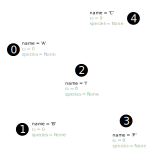
\includegraphics[width=7cm]{figureX1}
		\label{fig::X1}
	\end{subfigure}%
	\vline
	\begin{subfigure}{.5\textwidth}
		\centering
		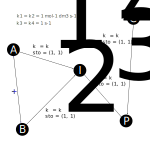
\includegraphics[width=7cm]{figureX2}
		\label{fig::X2}
	\end{subfigure}
	\caption{Reaction network node (a) and edge (b) initialisation for $s_1$.}
	\label{fig:network_init}
	\vspace{0.2cm}
\end{figure}

 Edges are then added for the addition of components ('+' edges) and reactions ('reaction' edges). Addition edges denote more than one component is required for a reaction, in $s_1$  there is one addition edge ($A$--$B$, represented with two directed edges $A \leftrightarrows B$). Reaction edges are added for species that convert from one into another and contain a rate constant $k$ and a stoichiometry (sto) change $(n, m)$. The full initialised \code{Network} for $s_1$ is shown in \figurename{ \ref{fig:network_init}b}, where for simplicity nodes are labelled with their name rather than index.
 
 The overabundant rate constants are initialised with $k = 1$ and a mapping generated to enable setting the unique rate constants i.e here $k_1 \equiv k_2$. A mapping is generated by, for each reaction edge, populating a list of edges that must have the same rate constant. These are neighbours over addition edges that also have reaction edges to the product and likewise over the addition edges of products.
 
 In $s_1$ stoichiometry changes are all $1 \rightarrow 1$ along the reaction edges. For a set $s_2 = \{2A \rightarrow B, A \rightarrow C\}$ stoichiometries are (2, 1) and (1, 1) for edges $A$--$B$ and $A$--$C$ respectively. When a system is assigned to a set of data initial concentrations are populated as the first in the \code{TimeSeries} of concentrations.

\section{Derivative}

Simulated kinetics ($c_i(t)$ for a component $i$ at a time $t$) are generated by numerical propagation of a set of ordinary differential equations (ODE) from the initial value of the concentrations using \emph{scipy}. The ODEs ($d\boldsymbol{c}/dt$, where $\boldsymbol{c}$ is the concentration vector) are constructed from the \code{Network} as follows.

For each node $i$ the change in concentration is the inflow minus the outflow

\begin{equation}
\frac{d c_i}{dt} = \text{inflows}(i) - \text{outflows}(i)
\end{equation}
\begin{equation}
\text{outflows}(i) = \sum_{j \in \{O_i\}} \frac{k_{i\rightarrow j}}{N_{n_j} + 1}\, a_i \,c_i^{a_i}\prod_{k \in \{n_i\rightarrow j\}} c_k^{a_k}
\end{equation}

where $\{O_i\}$ is the set of direct successor nodes to $i$, $k_{i \rightarrow j}$ is the rate constant from $i$ to $j$, $N_{n_j}$ is the number of neighbours along addition edges to node $j$, $a_i$ is the stoichiometry of $i$ along the $i$--$j$ reaction edge,  $c_i$ is the concentration of component $i$, $\{n_i \rightarrow j\}$ is the set of nodes which are neighbours to $i$ and also have a reaction edge to $j$. An example is shown in \figurename{ \ref{fig:outflows}}.

 \begin{figure}[h!]
	\vspace{0.2cm}
	\begin{subfigure}{.5\textwidth}
		\centering
		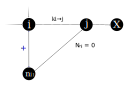
\includegraphics[width=7.5cm]{figureX4}
		\label{fig::X4}
	\end{subfigure}%
	\vline
	\begin{subfigure}{.5\textwidth}
		\centering
		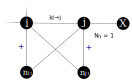
\includegraphics[width=7.5cm]{figureX3}
		\label{fig::X3}
	\end{subfigure}
	\caption{Visualisation of an outflow node $j$ originating from $i$.}
	\label{fig:outflows}
	\vspace{0.2cm}
\end{figure}

Likewise for the inflow nodes
\begin{equation}
\text{inflows}(i) = \sum_{j \in \{I_i\}} \frac{k_{j\rightarrow i}}{N_{n_j} + 1} a_i c_j^{a_j} \prod_{k \{n_j\rightarrow i\}} c_k^{a_k}
\end{equation}
where $j$ now enumerates over direct predecessor nodes of $i$, the set $\{I_i\}$. 










\end{document}